\begin{figure*}
 \centering
 % 115 classes
 \begin{minipage}[t]{0.45\linewidth}
 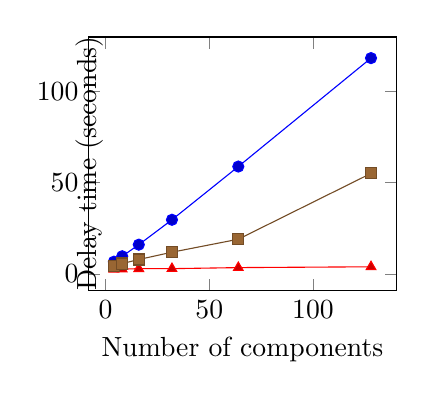
\begin{tikzpicture}
 \begin{axis}[
 	ylabel={Delay time (seconds)},
 	y label style={at={(0.08, 0.5)}},
 	xlabel={Number of components},width = 5.5cm,
 	height = 4.8cm]

 \addplot+[mark=*] coordinates
 	{(4,6.614953125) (8,9.60012962962963) (16,15.9376486486486) (32,29.564) (64,58.7045) (128,118.061571428571)};
 	
 \addplot+[mark=triangle*] coordinates
 	{(4,2.46368292682927) (8,2.56517142857143) (16,2.79086206896552) (32,2.81322222222222) (64,3.3868064516129) (128,3.83251724137931)};
 	
 \addplot+[mark=square*] coordinates
	 	{(4,4.31777777777778) (8,5.59077777777778) (16,7.81511538461538) (32,11.8165)  (64,18.9216363636364) (128,54.9538)};

 \end{axis}
 \end{tikzpicture}
 \caption{Delay time to detect fault with a\newline component size of 115 classes.\label{fig:delay-time-115}}
\end{minipage}
 % 4 classes
 \begin{minipage}[t]{0.45\linewidth}
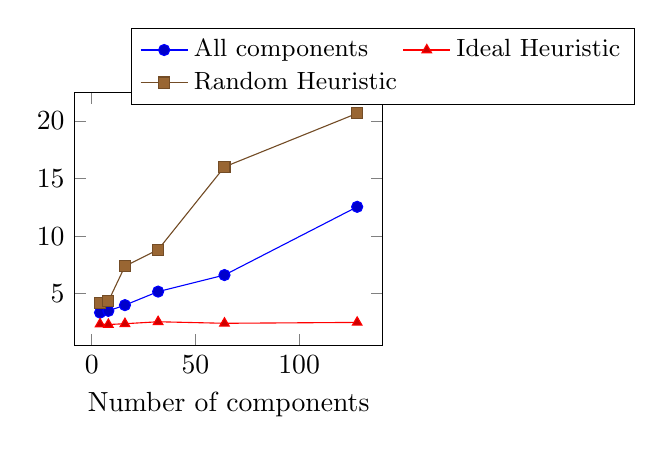
\begin{tikzpicture}
 \begin{axis}[
 	every axis legend/.append style={nodes={right}},
 	legend columns=2, 
 	legend style={at={(1.0,0.95)},
 	anchor=south,legend columns=1, font=\small},
 	xlabel={Number of components},width = 5.5cm,
 	height = 4.8cm]

 \addplot+[mark=*] coordinates
 	{(4,3.36101408450704) (8,3.51326153846154) (16,4.01246031746032) (32,5.18675) (64,6.62437704918033) (128,12.5490980392157)};
 	
 \addplot+[mark=triangle*] coordinates
 	{(4,2.3682619047619) (8,2.32882926829268) (16,2.39802777777778) (32,2.568) (64,2.43528571428571) (128,2.51225806451613)};
 	
 \addplot+[mark=square*] coordinates
	 	{(4,4.18407692307692) (8,4.35309090909091) (16,7.392) (32,8.82909090909091)  (64,16.017125) (128,20.6681428571429)};

	\legend{All components, Ideal Heuristic, Random Heuristic}
 \end{axis}
 \end{tikzpicture}
%\caption{4 classes}
 \caption{Delay time to detect fault with a\newline component size of four classes.\label{fig:delay-time-4}}
 \end{minipage}
\hspace{1cm}
\end{figure*}
